\documentclass[11pt]{article}
\usepackage{docstyle}
% Lesson 1 lost-mark points (from the material plus teaching observation), numbered once
\setcounter{lostmark}{0}
\lostmark{expand}{Differentiating brackets without expanding first: $(2x+1)(x-3)$ is not differentiated factor by factor.}
\lostmark{wrongfn}{Using the wrong function: the \kw{gradient} comes from $f'(x)$, the \kw{$y$-coordinate} comes from $f(x)$.}
\lostmark{terms}{Slips on simple terms: $7x \to 7$ (not $7x$ or $0$), and a constant $\to 0$.}
\lostmark{xinm}{Leaving $x$ inside the tangent's gradient: $y-y_{1}=(4x-3)(x-x_{1})$ is not a straight line. Substitute first.}
\lostmark{signs}{Sign slips with negative $x$: write $(-1)^{2}$ and $(-1)^{3}$ in brackets.}
\lostmark{nocalc}{``Use calculus'' ignored: $f'(x)$ must be written down. A calculator value alone does not show the method.}

\newlength\figunit
\begin{document}
\handouthead{Lesson 1 \textperiodcentered\ Gradients, Differentiation and Tangents}{NCEA Level 2 Mathematics \textperiodcentered\ AS 91262 Apply calculus methods in solving problems \textperiodcentered\ Handout}

\section{The one idea}\label{idea}
\begin{minipage}[c]{0.52\linewidth}
A straight line has one gradient. A curve does not: its steepness changes from point to point.
The \kw{gradient of a curve at a point} is the gradient of the \ttangent at that point
(the straight line that just touches the curve there).

\smallskip
\begin{keybox}
$f'(x)$ is a \kw{gradient machine}: put in an $x$-value, get out the gradient of the curve at that point.
\end{keybox}
For $y=x^{2}$ the gradient machine is $f'(x)=2x$. At A ($x=-1$) it gives $-2$ (going down),
at B ($x=1$) it gives $2$, and at C ($x=2$) it gives $4$ (steeper than at B).
\end{minipage}\hfill
\begin{minipage}[c]{0.44\linewidth}\centering
\setlength\figunit{8mm}
% y = x^2 with tangents at x = -1, 1, 2.  Tangent at x = a: y = 2a x - a^2 (computed).
% Caller sets \figunit.  Points A, B, C are at x = -1, 1, 2.
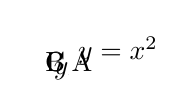
\begin{tikzpicture}[x=\figunit, y=0.6\figunit, line cap=round]
  \gridaxes{-3}{3}{-2}{6}{1}{2}{$y$}
  \begin{scope}
    \clip (-3,-2) rectangle (3,6);
    \curve{-2.5}{2.5}{\x*\x}
    \foreach \a/\pos in {-1/left, 1/right, 2/right}{
      \draw[line width=0.8pt, dashed] ({\a-0.9},{2*\a*(\a-0.9)-\a*\a}) -- ({\a+0.9},{2*\a*(\a+0.9)-\a*\a});
      \fill (\a,{\a*\a}) circle (2.2pt);
    }
  \end{scope}
  \node[anchor=south west] at (2.5,{2.5*2.5-0.2}) {$y=x^{2}$};
  % letters sit inside the parabola, above each tangent (checked):
  % A: x in [-0.95,-0.6], y in [1.1,1.9]; curve there is below 0.9 and tangent y=-2x-1 below 0.9
  % B: mirror of A;  C: x in [1.6,1.95], y in [4.1,4.9]; curve needs x > 2.02 at y = 4.1
  \node[anchor=south west, inner sep=1pt] at (-0.95,1.1) {A};
  \node[anchor=south east, inner sep=1pt] at (0.95,1.1) {B};
  \node[anchor=south east, inner sep=1pt] at (1.95,4.1) {C};
\end{tikzpicture}

\end{minipage}

\section{Words and symbols}\label{words}
\begin{tabular}{@{}p{0.30\linewidth}p{0.64\linewidth}@{}}
\toprule
\kw{gradient function} & the function that gives the gradient at every $x$. Also called the \kw{derivative}.\\
$f'(x)$ \enspace or\enspace $\dydx$ & two ways to write the \tgradfn. Say ``$f$ dash of $x$'' and ``$\mathrm{d}y$ by $\mathrm{d}x$''.\\
\kw{differentiate} & find the \tgradfn.\\
\kw{tangent} & the straight line touching the curve at one point, with the same gradient as the curve there.\\
\bottomrule
\end{tabular}

\section{Differentiating: the power rule}\label{rule}
\begin{keybox}
\[\ddx\bigl(a x^{n}\bigr)=a n\,x^{n-1}\qquad\text{multiply by the power, then take 1 off the power.}\]
\end{keybox}
Differentiate each term on its own.

\smallskip
\begin{tabular}{@{}llll@{}}
\toprule
term & what happens & \tderiv & why \\
\midrule
$x^{5}$ & power $5$ comes to the front, power becomes $4$ & $5x^{4}$ & rule \\
$4x^{3}$ & $4\times3=12$, power becomes $2$ & $12x^{2}$ & rule \\
$7x$ & $x=x^{1}$, so $7\times1\times x^{0}$ & $7$ & an $x$-term leaves its number \\
$9$ & a constant does not change & $0$ & a flat line has gradient $0$ \\
\bottomrule
\end{tabular}

\medskip
\kw{Expand brackets first.} The power rule works on single terms only.

\begin{example}{Worked example 1}
Differentiate $f(x)=3x^{4}-5x^{2}+7x-2$.
\begin{steps}
\item Term by term: $3x^{4}\to 12x^{3}$,\quad $-5x^{2}\to-10x$,\quad $7x\to7$,\quad $-2\to0$.
\item $f'(x)=\mathbf{12x^{3}-10x+7}$
\end{steps}
\end{example}

\begin{example}{Worked example 2}
Differentiate $y=(2x+1)(x-3)$.
\begin{steps}
\item Expand: $y=2x^{2}-6x+x-3=2x^{2}-5x-3$.
\item Differentiate: $\dydx=\mathbf{4x-5}$.
\end{steps}
Check: multiplying the derivatives of the brackets ($2\times1=2$) is wrong, see \lmnum{expand} below.
\end{example}

\section{Three question types}\label{types}
Read what is \emph{given} and what is \emph{asked}; that decides the route.

\smallskip
\begin{tabular}{@{}p{0.27\linewidth}p{0.37\linewidth}p{0.30\linewidth}@{}}
\toprule
given $\to$ asked & route & watch \\
\midrule
$x$ $\to$ gradient & differentiate, \kw{substitute $x$ into $f'(x)$} & not into $f(x)$ \\
gradient $\to$ point & \kw{solve $f'(x)=$ gradient} for $x$, then $y$ from $f(x)$ & a point needs $x$ and $y$ \\
gradient at $x$ $\to$ unknown constant & differentiate with the letter in, substitute $x$, set equal to the gradient, solve & the letter stays in $f'(x)$ \\
\bottomrule
\end{tabular}

\begin{example}{Worked example 3 \textperiodcentered\ gradient at a point}
Find the gradient of $f(x)=x^{3}-6x^{2}+4$ at the point where $x=5$.
\begin{steps}
\item $f'(x)=3x^{2}-12x$
\item $f'(5)=3(5)^{2}-12(5)=75-60=\mathbf{15}$
\end{steps}
\end{example}

\begin{example}{Worked example 4 \textperiodcentered\ point with a given gradient}
Find the point on $y=x^{2}-7x+1$ where the gradient is $3$.
\begin{steps}
\item $\dydx=2x-7$
\item $2x-7=3$, so $x=5$.
\item $y=5^{2}-7(5)+1=-9$.\quad The point is $\mathbf{(5,\,-9)}$.
\end{steps}
\end{example}

\begin{example}{Worked example 5 \textperiodcentered\ unknown constant (Merit step)}
The curve $f(x)=ax^{2}+3x-1$ has gradient $11$ at $x=2$. Find $a$.
\begin{steps}
\item $f'(x)=2ax+3$\quad (treat $a$ like a number)
\item $f'(2)=4a+3=11$
\item $4a=8$, so $\mathbf{a=2}$.\quad Check: $f'(2)=2(2)(2)+3=11$.
\end{steps}
\end{example}

\section{Equation of a tangent}\label{tangent}
\subsection{Write it in this order}
\begin{enumerate}[leftmargin=7mm, itemsep=1pt]
\item \kw{Point}: $x_{1}$ is given; find $y_{1}$ from $f(x)$.
\item \kw{Gradient}: $m=f'(x_{1})$, a number.
\item \kw{Line}: $y-y_{1}=m(x-x_{1})$, then rearrange to $y=mx+c$.
\end{enumerate}

\begin{example}{Worked example 6}
Find the equation of the tangent to $y=x^{3}-2x+1$ at $x=2$.
\begin{steps}
\item Point: $y=2^{3}-2(2)+1=5$, so $(2,\,5)$.
\item Gradient: $\dydx=3x^{2}-2$, so $m=3(2)^{2}-2=10$.
\item Line: $y-5=10(x-2)$, so $\mathbf{y=10x-15}$.
\end{steps}
\end{example}

\begin{example}{Worked example 7 \textperiodcentered\ two unknowns (Merit)}
The curve $y=ax^{2}+bx$ passes through $(1,\,5)$, and its gradient at that point is $8$. Find $a$ and $b$.
\begin{steps}
\item On the curve: $a(1)^{2}+b(1)=5$, so $a+b=5$.
\item Gradient: $\dydx=2ax+b$; at $x=1$: $2a+b=8$.
\item Subtract: $a=3$, then $b=2$.\quad $\mathbf{a=3,\ b=2}$.
\end{steps}
Two unknowns need two equations: one from the \kw{point}, one from the \kw{gradient}.
\end{example}

\textbf{Parallel lines have equal gradients.} ``The tangent is parallel to $y=2x+1$'' means $f'(x)=2$.

\section{What each grade looks like here}\label{grades}
\begin{tabular}{@{}p{0.14\linewidth}p{0.80\linewidth}@{}}
\toprule
Achieved & apply one method: differentiate and find a gradient, or find a tangent at a given $x$.\\
Merit & link steps (relational thinking): find an unknown constant from a gradient, use two conditions for two unknowns, use a parallel line.\\
Excellence & extended abstract thinking: e.g.\ a tangent through an outside point, or where a tangent meets the curve again, written as a full chain of reasoning.\\
\bottomrule
\end{tabular}

\section{Checking with the fx-9750GIII}\label{calc}
\begin{itemize}[leftmargin=5mm, itemsep=1pt]
\item \kw{Gradient at a point}: \textsf{RUN-MATRIX} $\to$ \textsf{OPTN} $\to$ \textsf{CALC} (F4) $\to$ $\mathrm{d}/\mathrm{d}x$ (F2).
Type the function in $X$, a comma, then the $x$-value: e.g.\ $\mathrm{d}/\mathrm{d}x(X^{3}-2X+1,\,2)$ gives $10$.
\item \kw{Solving a quadratic}: \textsf{EQUA} $\to$ \textsf{POLY} (F2) $\to$ degree $2$, enter the coefficients.
\item The calculator checks the answer. The written $f'(x)$ is what shows the method.
\end{itemize}

\section{Ways to lose marks}\label{lose}
From the material plus teaching observation.
\begin{enumerate}[label=\textbf{\arabic*.}, leftmargin=7mm, itemsep=2pt]
\item[\textbf{\lmnum{expand}}] \lmtxt{expand}
\item[\textbf{\lmnum{wrongfn}}] \lmtxt{wrongfn}
\item[\textbf{\lmnum{terms}}] \lmtxt{terms}
\item[\textbf{\lmnum{xinm}}] \lmtxt{xinm}
\item[\textbf{\lmnum{signs}}] \lmtxt{signs}
\item[\textbf{\lmnum{nocalc}}] \lmtxt{nocalc}
\end{enumerate}
\end{document}
